% \iffalse
\let\negmedspace\undefined
\let\negthickspace\undefined
\documentclass[journal,12pt,twocolumn]{IEEEtran}
\usepackage{cite}
\usepackage{amsmath,amssymb,amsfonts,amsthm}
\usepackage{algorithmic}
\usepackage{graphicx}
\usepackage{textcomp}
\usepackage{xcolor}
\usepackage{txfonts}
\usepackage{listings}
\usepackage{enumitem}
\usepackage{mathtools}
\usepackage{gensymb}
\usepackage{comment}
\usepackage[breaklinks=true]{hyperref}
\usepackage{tkz-euclide} 
\usepackage{listings}
\usepackage{gvv}                                        
\def\inputGnumericTable{}                                 
\usepackage[latin1]{inputenc}                               \usepackage{caption}
\usepackage{color}                                            
\usepackage{array}                                            
\usepackage{longtable}                                       
\usepackage{calc}                                             
\usepackage{multirow}                                         
\usepackage{hhline}                                           
\usepackage{ifthen}                                           
\usepackage{lscape}

\newtheorem{theorem}{Theorem}[section]
\newtheorem{problem}{Problem}
\newtheorem{proposition}{Proposition}[section]
\newtheorem{lemma}{Lemma}[section]
\newtheorem{corollary}[theorem]{Corollary}
\newtheorem{example}{Example}[section]
\newtheorem{definition}[problem]{Definition}
\newcommand{\BEQA}{\begin{eqnarray}}
\newcommand{\EEQA}{\end{eqnarray}}
\newcommand{\define}{\stackrel{\triangle}{=}}
\theoremstyle{remark}
\newtheorem{rem}{Remark}
\begin{document}

\bibliographystyle{IEEEtran}
\vspace{3cm}

\title{Audio Filtering}
\author{EE23BTECH11013 - Avyaaz$^{*}$% <-this % stops a space
}
\maketitle
\newpage
\bigskip

\renewcommand{\thefigure}{\arabic{figure}}
\renewcommand{\thetable}{\arabic{table}}

\bibliographystyle{IEEEtran}

\begin{table}[htbp]
\setlength{\extrarowheight}{8pt}
\centering
 
\begin{tabular}{|c|c|}
\hline
\textbf{Parameter} & \textbf{Description}\\
\hline 
$x(n)$ & Input audio signal \\
\hline
$y(n)$ & Output audio signal\\
\hline
$H(e^{j\omega})$& Discret Time Fourier Transform of
$x(n)$\\
\hline
$h(n) $& Impulse response \\
\hline
\end{tabular}



 \caption{Parameters}
\label{tab:parameters}
\end{table}

\begin{figure}[htbp] 
\centering
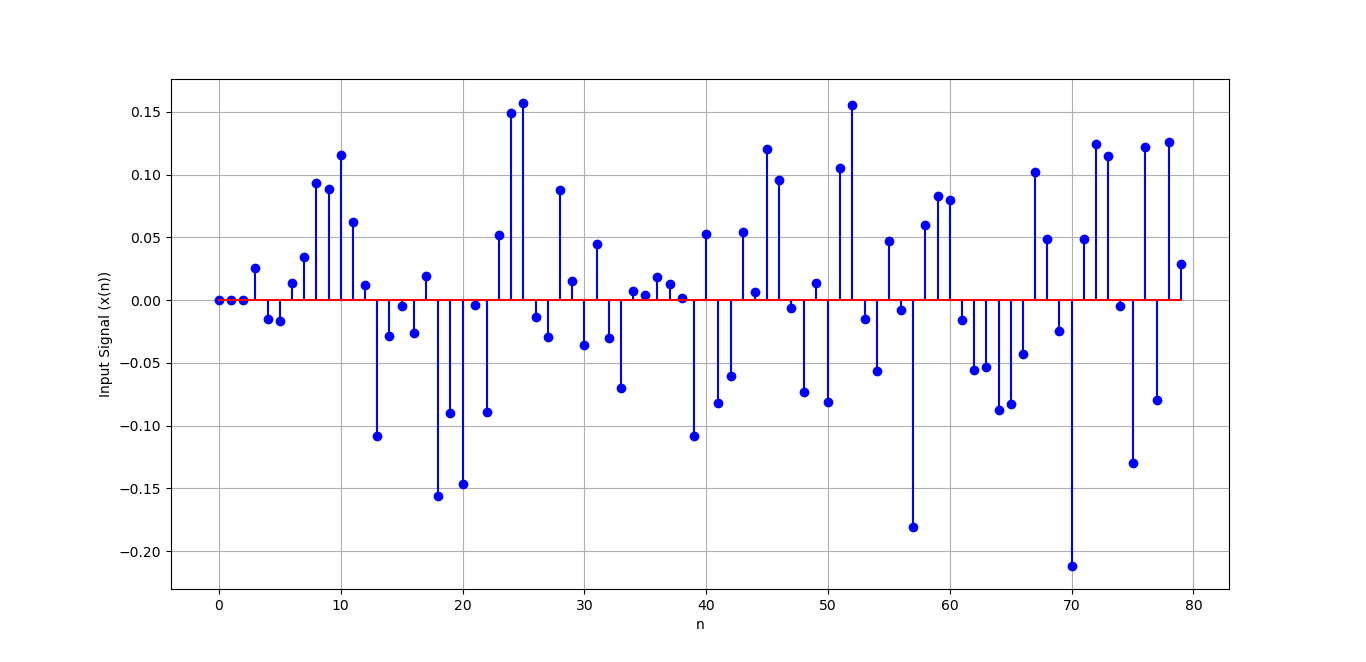
\includegraphics[width=\columnwidth]{figs/x(n).png}
\caption{Plot of $x(n)$  vs $n$ }
\end{figure}
Output audio signal can be obtained from the difference equation: 
\begin{align}
     \sum _{m=0}^{M}a\brak{m}y\brak{n-m}=\sum _{k=0}^{N}b\brak{k}x\brak{n-k}
\end{align}
where, 
coefficients of $a$ and $b$ are obtained from the 'noise\_reduction.py'
\begin{figure}[htbp] 
\centering
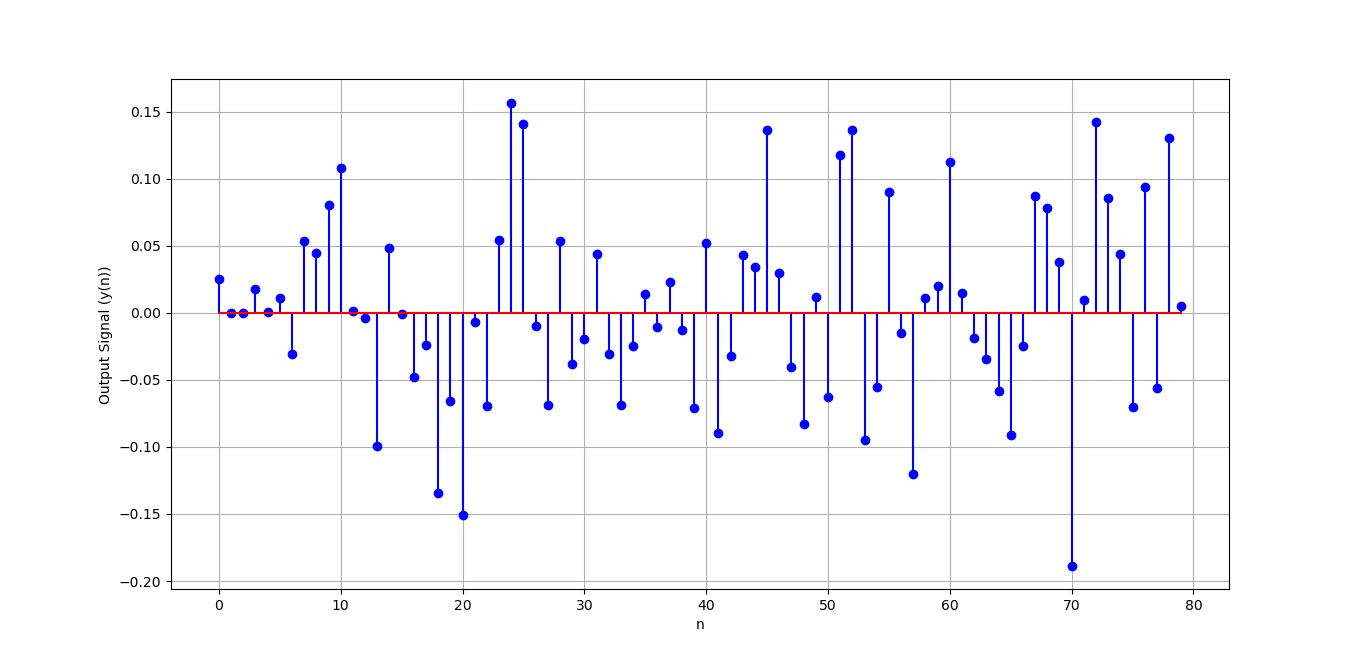
\includegraphics[width=1.1\columnwidth]{figs/y(n).png}
\caption{Plot of $y(n)$ vs $n$}
\end{figure}\\
Here,
\begin{align}
x[n] & \system{\mathcal{F}}X(\omega) \\
y[n] & \system{\mathcal{F}}Y(\omega) \\
h[n] & \system{\mathcal{F}}\frac{Y(\omega)}{X(\omega)} = H(\omega)
\end{align}
\begin{figure}[htbp] 
\centering
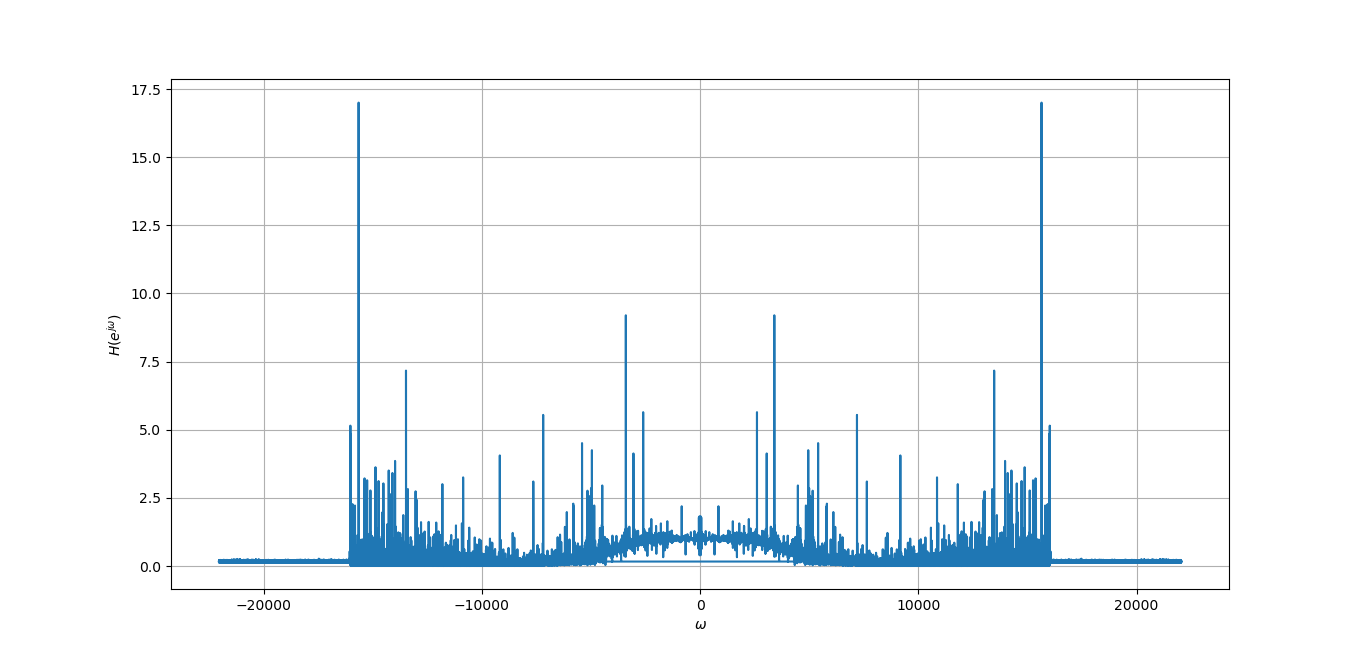
\includegraphics[width=\columnwidth]{figs/H(z).png}
\caption{Plot of $|H(e^{j\omega})|$ vs $\omega$}
\end{figure}\\
Here,

$h(n)$ is inverse fourier transform of $H(\omega)$
\begin{align}
    H(\omega) \mathrel{\substack{\mathcal{F}^{-1}\\\longleftrightarrow}} h(n)
\end{align}

\begin{figure}[htbp] 
\centering
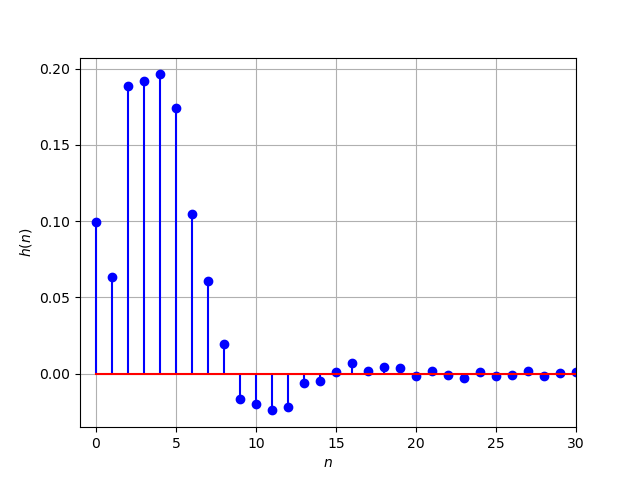
\includegraphics[width=\columnwidth]{figs/h(n).png}
\caption{Plot of $h(n)$ vs $n$}
\end{figure}


\end{document}
